\documentclass{article}
\usepackage[T1]{fontenc}
\usepackage[utf8]{inputenc}
\usepackage[brazil]{babel}
\usepackage{graphicx}

\author{Tiago Royer}
\title{Instance Based Learning}

\newcommand{\kNN}{k\mathit{NN}}

\begin{document}

\maketitle

\section{Introdução}

Os algoritmos IBL (\emph{Instance Based Learning})
são uma coleção de algoritmos simbólicos
que classificam instâncias baseados num conjunto de treinamento.
Ao contrário de usar apenas $\kNN$,
os algoritmos IBL tentam identificar apenas os aspectos mais relevantes
do conjunto de treinamento,
simultaneamente reduzindo o tamanho do descritor conceitual
e tolerando ruído na entrada.

Este relatório descreve como e quais algoritmos foram implementados
e discute alguns resultados.

\section{Estrutura do Repositório}

Este repositório é um conjunto de ferramentas de linha de comando
que trabalham com datasets. Há programas para visualização,
geração, e classificação de dados a partir destes datasets.

A maior parte dos programas precisa ser compilada.
O makefile do repositório está configurado
para respeitar a variável \texttt{CXXFLAGS},
portanto os programas do repositório pode ser compilado com
\begin{verbatim}
    $ CXXFLAGS=-O2 make
\end{verbatim}

Todos os programas suportam a opção \verb|--help| na linha de comando.

\subsection{Arquivos \texttt{.data}}

Estes são os conjuntos de dados utilizados pelos programas deste repositório.
São arquivos de texto com uma estrutura específica,
que está detalhada no arquivo \verb|datasets/format.md|.
A maior parte dos programas ou leem datasets da entrada padrão
ou geram conjuntos de dados para a entrada padrão.
(A exceção é o \verb|classify|, em que o conjunto de dados
deve ser especificado na linha de comando através da opção \verb|--dataset|.)

O repositório vem com dois conjuntos de dados prontos.
O primeiro, \verb|datasets/iris.data|,
é o conhecido conjunto de dados de flores do gênero \emph{Iris}%
\footnote{
    \texttt{http://en.wikipedia.org/wiki/Iris\_flower\_data\_set}.
}.
O segundo, \verb|datasets/enclave.data|,
pode ser visto na figura \ref{enclave}.

\begin{figure}[h]
    \centering
    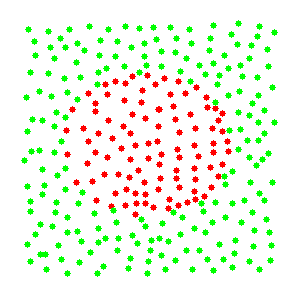
\includegraphics[scale=0.5]{enclave.png}
    \caption{Conjunto de dados \texttt{datasets/enclave.data}.}
    \label{enclave}
\end{figure}

Existem também dois programas para gerar conjuntos de dados.

\texttt{datatools/generate\_spiral} gera espirais bidimensionais.
O programa permite controlar parâmetros como o número de espirais geradas.

\texttt{pixel\_chooser --generate-dataset --blank 500 500} abre uma janela em branco,
de 500 por 500 pixels, e espera que o usuário clique em algumas posições.
As posições clicadas virarão os pontos no conjunto de dados.
Apertando barra de espaço, a classe dos pontos é alterada;
apertanto qualquer outra tecla encerra o programa e imprime o conjunto gerado.
(Foi assim que foi construído o conjunto \texttt{enclave.data}.)

\section{Programas para classificação de dados}

Apenas dois programas no repositório lidam diretamente com IBL.
O programa \texttt{ibl}, na raíz do repositório,
exibe uma janela dividida em três telas.
A primeira mostra o dataset de entrada;
a segunda mostra o descritor conceitual restante após rodar o algoritmo IBL,
e a última mostra as áreas de influência do descritor conceitual.

O programa \texttt{ibl} permite apenas visualizar
o resultado da execução dos algoritmos IBL.
Entretanto, ele não permite classificar novos pontos
usando o descritor conceitual gerado.
O programa \texttt{classify} é o oposto disso:
ele não possui nenhuma funcionalidade de visualização
(ele funciona em modo \emph{batch}),
mas permite que novas instâncias sejam classificadas
contra o descritor conceitual resultante.

Todas as opções da linha de comando do \texttt{ibl}
são aplicáveis a \emph{classify}, portanto iremos descrevê-las apenas no primeiro.

Para rodar um exemplo com IBL 2, podemos executar
\begin{verbatim}
    $ ./ibl --ibl 2 --shuffle --noise 10 < datasets/enclave.data
    --shuffle-seed 3456 --noise-seed 13456
\end{verbatim}
O programa deve reportar, na saída padrão, 245 acertos e 65 erros,
e exibir a imagem \ref{iblimg}.

\begin{figure}[h]
    \centering
    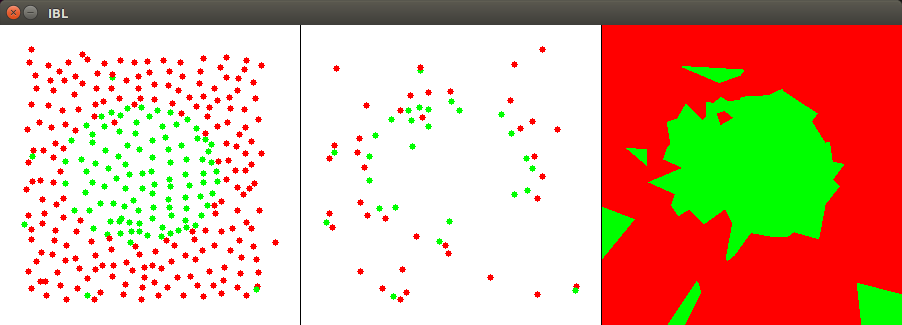
\includegraphics[scale=0.3]{ibl.png}
    \caption{Execução de IBL 2 no conjunto de dados \texttt{enclave.data}.}
    \label{iblimg}
\end{figure}
\end{document}
